
%*****************************************
\chapter{Realisierung}\label{ch:Realisierung}
%*****************************************
    Bei der Realisierung einer AIDS müssen wie in~\autoref{ch:Grundlagen} beschrieben zwei Phasen durchlaufen werden.
    Die Trainingsphase und die Testphase.
    Diesen beiden Phasen liegt allerdings schon ein präparierter Datensatz und die Definition der exakten Eingaben und Ausgaben des \ac{LSTM} zu Grunde. 
    Welche Datensätze überhaupt in Frage kommen wurde bereits in~\autoref{sec:Datensatz} untersucht.
    Wie dieser weiterverarbeitet, für das \ac{LSTM} vorbereitet wird und welche Informationen neben dem Namen des System Calls verwendet werden kann, 
    soll in~\autoref{sec:Preprocessing} betrachtet werden.
    Zuvor in~\autoref{sec:Tools} werden verschiedene Tools betrachtet, die für die Vorverarbeitung und weitere Implementierungen nötig sind.
    Der eigentliche Algorithmus, also das Finden von Anomalien in den Daten wird dann im~\autoref{sec:Algorithmus} beschrieben.
    Nachdem so also der verarbeitende Teil betrachtet wurde, soll in~\autoref{sec:StrukExp} die Strukturierung der Experimente präsentiert werden.
    Diese Strukturierung hat zum Ziel früh wenig vielversprechende Konfigurationen auszuschließen um ressourcenschonend Auswertungen durchzuführen.
    Speziell die Ressource Zeit, wie sich später zeigen wird, ist dabei im Rahmen dieser Arbeit eine Entscheidende.
    Abschließen soll dieses Kapitel dann in~\autoref{sec:Metriken} die Untersuchung von Metriken, welche dann für die Auswertung der Experimente benötigt wird.



    \section{Verwendete Tools}\label{sec:Tools}
        Tensorflow Keras
        Rechencluster clara
        sysdig

    \section{Vorverarbeitung}\label{sec:Preprocessing}
        %In dem kommenden Abschnitt~\ref{sec:struktur} wird die erste Vorverarbeitung des Datensatzes vorgestellt.
        Im kommenden Abschnitt~\ref{sec:syscalldarstellung} soll untersucht werden, welche Darstellungsformen für die eigentlichen System Calls interessant und sinnvoll sind.
        In dieser Arbeit werden die System Call Daten als Datenstream betrachtet.
        Weshalb in Abschnitt~\ref{sec:streamdarstellung} die Frage geprüft, wie dieser für das \ac{LSTM} dargestellt wird.
        Ein weiterer wichtiger Teil der Arbeit besteht darin, zu klären welche Metadaten neben dem Namen des System Calls noch verwendet werden können,
        um die Erkennungsrate zu erhöhen, bzw.\ die Fehlerrate zu verringern.
        Die Frage welche Informationen dafür verwendet werden können und wie diese dargestellt werden, soll in Abschnitt~\ref{sec:Meta}

        %\subsection{Vorverarbeitung des Datensatzes}\label{sec:struktur}
            %Gegeben 10 szenarien die aus bekannten CVEs bestehen.\
            %mit ca. 1000 files durschnittlich 45sec
            %in runs.csv genauere beschreibung files mit label und zeitangabe falls exploit
            %falls kein exploit dann exploit start time -1
            %keine dauer des exploits also ende nicht bekannt 
            %nicht systemcall genau start des angriffs angegeben 
            %führe puffer ein, da angegebener Zeitpunkt ungenau, sodass auch wirklich jeder angriff nach exploit start time
            %alles nach dem angrffszeitpunkt muss als anomalie gewertet werden, auch wenn angriff evtl noch nicht gestartet hat oder schon vorbei.
            %%TODO Quadranten
            %filtern von switch statements in Datensatz weil keine system calls
            %nur schließende syscalls keine öffnenden.
            %Muss wie in~\ref{sec:syscalls} beschrieben immer beide geben.
            %Schließende interessant, da auch Rückgabewerte betrachtet werden können

        \subsection{Darstellung eines System Calls}\label{sec:syscalldarstellung}
            Neuronale Netze benötigen numerische werte deswegen Umwandlung von Namen der System Calls. 
            Eine einfache Kodierung dieser Strings bestünde darin die System Calls in Integer Werte umzuwandeln.
            Allerdings entstehen dabei künstliche Zusammenhänge und Ordnungen, welche für den Lernvorgang unvorteilhaft sein können~\cite{NEURALBISHOP1995}.
            Werden die System Calls als kategorische Daten betrachtet bietet sich das für neuronale Netze typische \ac{OHE} an.
            \paragraph{One-Hot-Encoding}
                Für die Darstellung eines System Calls mit dem \ac{OHE}, muss zunächst die Anzahl $n$ der unterschiedlichen System Calls ermittelt werden.
                Der System Call $sc_i$ aus der Menge der möglichen System Calls $ SC = \{sc_1,sc_2,\dots,sc_k\}$ 
                wird dann als Bit-Vektor $v_i$ der Länge $k$ kodiert.
                Dabei nehmen alle Stellen bis auf $i$ den Wert $0$ an und dort den Wert $1$.
                So wird aus dem System Call \textit{open} aus der Menge $SC = \{open, close, read\}$ der Vektor $v_1 = (1, 0, 0)$
                Da die Anzahl der möglichen System Calls und damit auch $n$ begrenzt ist, scheint diese Darstellung für einen System Call denkbar.
                Allerdings bringt sie auch zwei neue Probleme mit sich.
                Zum einen führt das \ac{OHE} eines System Calls bei großem $k$ zu einem langen und spärlich besetzten Vektor $v_i$.
                Gerade bei neuronalen Netzen führt das zu längeren Rechenzeiten.
                Und der neu gewonnen Vorteil, dass keine künstlichen Ordnungen vorhanden ist birgt den Nachteil, dass tatsächlich ebenso vorhandene Zusammenhänge verloren gehen.
                So besteht mindestens ein semantischer Zusammenhang zwischen \textit{open} und \textit{close} in der englischen Sprache, dieser ist in dem \ac{OHE} verloren gegangen. 
                Optimaler Weise gilt es also eine Darstellung zu finden die kurz ist und in der nur gewollte Ordnungen vorhanden sind.
                In der \ac{NLP} gilt es ähnliche Probleme durch die Darstellungen der Wörter zu lösen, zum Beispiel mit dem \ac{W2V} Verfahren.

            \paragraph{Word2Vec}
                Das \ac{W2V} Verfahren ist ein auf feedforward neuronalen Netzen basierender Ansatz, welcher häufig in der \ac{NLP} eingesetzt wird~\cite{W2VAYYADEVARA2018}.
                Dabei werden Wörter aus einem gegebenen Satz an möglichen Wörtern anhand eines Trainingsdatensatzes in dichte Vektoren $v_{w2v}$ fester Länge $e$ kodiert beziehungsweise \textit{embedded}\marginpar{zu dt.\ eingebettet}.
                Also ein System Call $sc_i$ aus der Menge $SC = \{sc_1,sc_2,\dots,sc_n\}$ wird umgewandelt in einen Vektor $v_{w2v}$ mit gegebener Länge $e$.
                Ziel des von~\cite{W2VMIKOLOV2013} eingeführten \ac{W2V} Verfahrens ist es eine Dimensionsreduktion durchzuführen, bei welcher möglichst viel Kontextinformationen erhalten bleiben.
                So sollen also die Vektordarstellungen von ähnlichen Wörtern ebenso ähnlich sein.
                Dies wird erreicht, indem Worte für das Erstellen der Kodierung nicht einzeln betrachtet werden, sondern immer in einem Kontext.
                Es wird angenommen, dass Wörter die häufig in einem ähnlichen Kontext auftreten, auch ähnlich sind.
                Dabei ist mit Kontext die Wörter vor und nach dem aktuellen Wort gemeint.
                Wie umfangreich dieser Kontext für jedes Wort sein soll, wird mit der Fenstergröße $w$ festgelegt.

                In der Trainingsphase gibt es zwei verschiedene Ansätze, zum einen das \textit{Continuous Bag-Of-Words},
                dabei wird versucht eine Vorhersage über ein Wort anhand des Kontextes zu machen.
                Hingegen wird unter Verwendung von \textit{Skip-gram}, eine Vorhersage des Kontextes aufgrund des Wortes vorgenommen.~\cite{EMBEDDINGPILEHVAR2020}

                Schwierigkeiten wie das häufige auftreten von Wörtern in der englischen Sprache wie \textit{the}, treten in der System Call Domäne nicht auf.
                Die Vorteile der dichtbesetzten und dimensionsreduzierten Vektoren machen sich auch bereits~\cite{IDSTHREADGRIMMER2021} in der anomaliebasierten \ac{HIDS} mit System Calls zu nutzen.

                %TODO
                {\color{red} TODO Wunderlich einbinden}
                Wie in \cite{W2VWUNDERLICH2019} beschrieben \ac{OHE} pot. besser, aber Dimensionsreduktion entscheidend.
                Zeitlicher Vorteil überwiegt in dieser Arbeit weshalb dieses Embedding auch im Folgenden verwendet.
                
                Neben den eigentlichen Namen der System Call enthalten tatsächliche System Calls wie in \autoref{sec:syscalls} beschrieben noch wesentlich mehr Informationen.
                Wie zumindest Teile dieser die Embeddings der System Calls erweitern können soll im folgenden Abschnitt untersucht werden.

        \subsection{Darstellung weiterer Parameter}\label{sec:Meta}
                Wie zusätzliche Informationen der System Calls genutzt werden können ist auch Gegenstand bestehender Forschung.
                In \autoref{sec:related_sys_arg} wurden die verschiedenen bestehenden Ansätze untersucht.
                Im Folgenden soll es speziell darum gehen neue Darstellungsformen der System Call Argumente zu finden.
                Dabei soll noch einmal kurz auf die in \autoref{sec:syscalls} besprochenen Grundlagen zurückgegriffen werden um einen ersten Anhaltspunkt für wichtige Informationsquellen zu finden.

                Um die Unterscheidung von Normalverhalten und einer Anomalie zu erleichtern, müssen Faktoren betrachtet werden, welche sensibel auf eine Veränderung des Normalverhaltens reagieren.
                Gleichzeitig sollen dabei aber nicht einzelne Angriffe genutzt werden um diese Faktoren zu ermitteln.
                Denn dabei besteht die Gefahr Signaturen einzelner Angriffe abbilden zu wollen, was wie in \autoref{sec:Datenanalyse} ungewollte Nachteile hat.
                Ziel dieses Abschnitts ist es die Überlegungen und Umsetzungen von zwei Verfahren zur Darstellung von zusätzlichen System Call Informationen zu präsentieren.

                \paragraph{Zeitliche Abstände von System Calls}

                    Wie bereits in \autoref{sec:related_sys_arg} beschrieben verwenden Lucket et al.~\cite{TIMINGLUCKETT2016} die Timing-Information von System Calls für das Aufspüren von Rootkits.
                    In diesem Abschnitt wird diese Idee wieder aufgegriffen.
                    Die Grundidee besteht darin, dass durch ein Angriffsverhalten eine zumindest kurzzeitige Veränderung im Timing der auftretenden System Calls eintritt.
                    Dabei gelten System Calls in diesem Ansatz nur als aufeinanderfolgend, sofern sie auch aus dem selben Thread stammen.
                    Eine genauere Erläuterung dazu erfolgt in \autoref{sec:streamdarstellung}.
                    Um den Unterschied in den Normaldaten und Angriffsdaten zu untersuchen wurden in \autoref{fig:time_delta} die zeitlichen Abstände zwischen aufeinanderfolgenden System Calls aus dem Bruteforce und dem CVE-2019-5418 Szenario des \ac{LID-DS} geplottet.
                    In Blau sind die Abstände der System Calls während des Normalverhaltens eingetragen und in Rot die des Normalverhaltens mit zusätzlichen Angriffsverhalten.
                    Im rechten Plot kein sichtlicher Unterschied zwischen Angriffsverhalten und dem Normalverhalten zu erkennen.
                    Der in diesem Szenario durchgeführte Angriff scheint nicht zu einer Abweichung der Zeitabstände zwischen System Calls zu führen.
                    Im linken Plot hingegen ist eine Abweichung im Bereich ab ca. $0.05*10^{6}$\textit{ns} zu erkennen.

                    %Wie in \autoref{sec:related_no_arg} beschrieben können Verfahren die keine weiteren Parameter verwenden umgangen werden, indem weitere System Calls eingefügt werden~\cite{Syscallseqexploit1}.
                    \begin{figure}
                        \centering
                        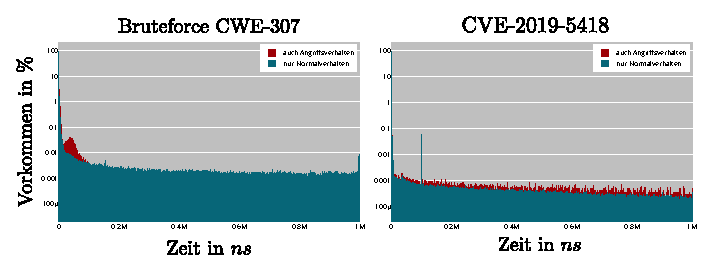
\includegraphics[width=\textwidth]{images/CVE-2012--Test-data-time_delta.eps}
                        \caption{Dargestellt ist der zeitliche Abstand zwischen zwei System Calls aus dem selben Thread.
                                 Diese werden in ihrer Häufigkeit in Prozent an allen auftretenden Abstände in dem Plot eingetragen.
                                 Verwendet wurden dafür nur die Testdaten. Links für das Bruteforce Szenario und rechts für das CVE-2019-5418 Szenario.
                                 Blau: Nur Normalverhalten, Rot: Normalverhalten und Angriffsverhalten}
                        \label{fig:time_delta}
                    \end{figure}

                    Die Umsetzung der beschriebenen Idee wird erreicht indem der zeitlichen Abstand $\tau$ zwischen zwei aufeinanderfolgenden System Calls berechnet wird und diesen als weiteren Eingabeparameter für den verarbeitenden Algorithmus verwendet wird.
                    In der Trainingsphase wird zunächst nur der größte Abstand $\tau_{max}$ aus den Trainingsdaten ermittelt.
                    Mithilfe dieses Wertes werden dann in der Testphase alle Werte wie in \autoref{eq:time_norm} beschrieben normalisiert.
                    \begin{equation}\label{eq:time_norm}
                        \tau_{norm} = \frac{\tau}{\tau_{max}}
                    \end{equation}
                    So gilt für die meisten Werte $\tau_{norm}=[0;1]$.
                    Falls $\tau\geq\tau_{max}$ gilt, kann dieser Wert auch größer als $1$ werden.

                    Doch treten mit der Verwendung dieser Information als Extraparameter zwei Probleme auf.

                    Zum einen stellt sich die Frage, ob eine Verbesserung eines Szenarios mit abweichenden Abständen\marginpar{zw. Normal- und Angriffsverhalten} eine Verschlechterung in Szenarien in welchen dies nicht der Fall ist zur Folge hat.
                    Und zum anderen stellt sich die generelle Frage ob diese Information den möglichen Ergebnisraum wesentlich vergrößert worunter die Ergebnisqualität im Gesamten leidet.
                    Denn das Betriebssystem selbst beeinflusst die Timings der System Calls, so könnten Informationen eingebettet werden welche wenig Aussagekraft über das Normalverhalten eines Prozesses haben.
                    Ob dies das Lernen des Normalverhaltens verbessert oder verschlechtert wird in \autoref{sec:Ergebnis_timing} untersucht.
                    %\begin{figure}
                        %\centering
                        %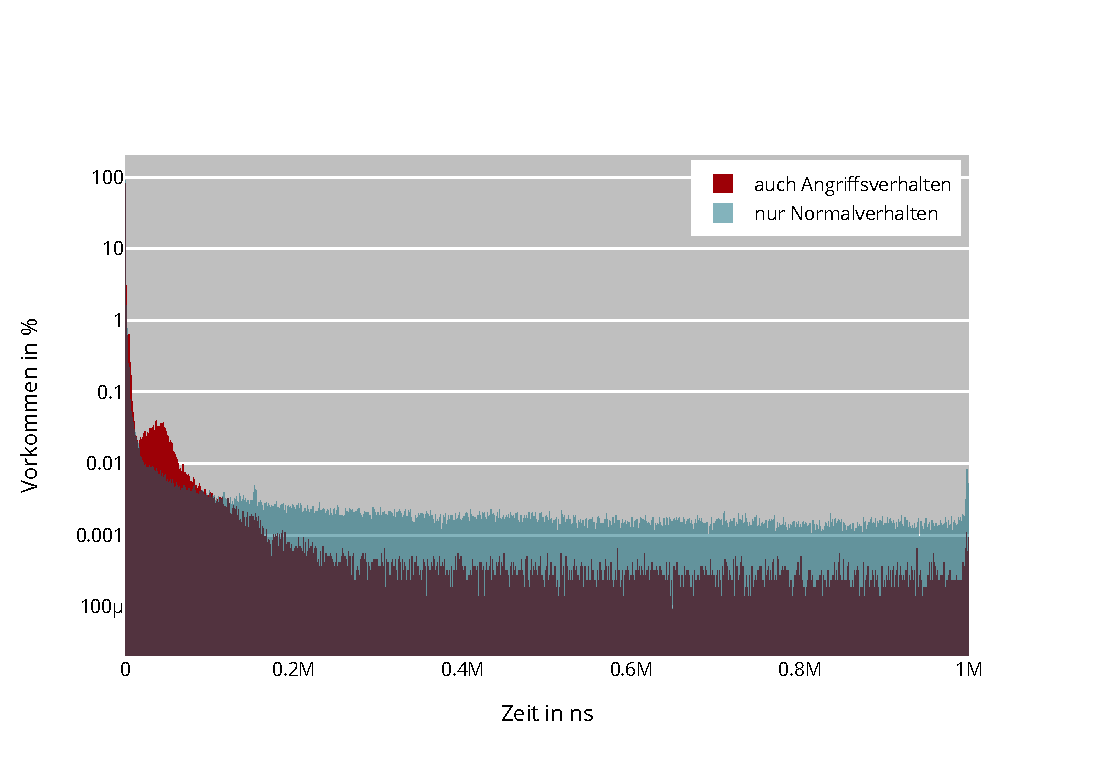
\includegraphics[width=\textwidth]{images/CVE-2012--Test-data-time_delta.pdf}
                        %\caption{Dargestellt ist der zeitliche Abstand zwischen zwei System Calls aus dem selben Thread.
                                 %Diese werden in ihrer Häufigkeit in Prozent an allen auftretenden Abstände in dem Plot eingetragen.
                                 %Verwendet wurden dafür nur die Testdaten des 
                                 %Blau: Nur Normalverhalten}
                        %\label{fig:time_delta_werte}
                    %\end{figure}

                \paragraph{Return Werte}

                    Wie in \autoref{sec:syscall_allg} angemerkt, besteht ein System Call aus zwei \glqq Phasen\grqq.
                    Wobei die zweite Phase den Rückgabewert des Betriebssystemskernel beinhaltet.
                    Bei erfolgreicher Durchführung ist dieser Rückgabewert positiv, ansonsten negativ.
                    So gibt der Rückgabewert eines \textit{write} System Calls an wieviele Bytes gelesen wurden.
                    Der Rückgabewert enthält in diesem Beispiel also wertvolle Informationen über den tatsächlichen Ablauf des spezifischen System Calls.
                    Auch weitere schreibende und lesende System Calls geben die gelesene oder geschriebene Bytes zurück.
                    Für manche System Calls die im Zusammenhang mit Sockets stehen gilt dies ebenfalls.
                    Deswegen soll in diesem Abschnitt die Kodierung von System Call Rückgabewerten betrachtet werden welche Daten schreiben oder lesen und Daten über Sockets empfangen oder senden. 
                    Dabei wurden nur System Calls betrachtet, die auch im Datensatz vorkommen und einen Byte Rückgabewert haben.
                    Leider fallen dabei System Calls wie \textit{send} heraus, da der Rückgabewert die Anzahl der gesendeten Charaktere angibt und nicht die Anzahl an geschriebenen Bytes.
                    In \autoref{tab:syscall_return} werden die ausgewählten System Calls mit einer Kurzbeschreibung vorgestellt.

                    \begin{table}[ht]
                        \small
                        \centering
                        \begin{tabular}{cp{6cm}p{3cm}}
                            \hline
                            \rowcolor{GruvGray!36}
                            \multicolumn{3}{c}{System Calls}\\
                            \hline
                            Name & Beschreibung & Rückgabewerte\\
                            \hline
                            \hline
                            \rowcolor{GruvGray!16}
                            %open& Öffnet die von \textit{pathname} spezifizierte File. Falls diese nicht existiert kann sie mit dem Zusatz \textit{O_CREAT} automatisch erstellt werden & path, asdklfjs, slddk\\
                            write   & Schreibt bis zu \textit{count} Bytes aus dem Buffer (ab Stelle \textit{buf}) in die Datei, welche über den Filedeskriptor $fd$ definiert wird. & Geschriebene Bytes oder $-1$ bei Fehler\\
                            pwrite  & Schreibt bis zu \textit{count} Bytes aus dem Buffer (ab Stelle \textit{buf}) in die Datei, welche über den Filedeskriptor $fd$ definiert wird. Dabei wird der Datei Offset nicht geändert.& Geschriebene Bytes oder $-1$ bei Fehler\\
                            \rowcolor{GruvGray!16}
                            writev  & Schreibt \textit{iovcnt} Vektor in die Datei, welche über den Filedeskriptor $fd$ definiert wird.& Geschriebene Bytes oder $-1$ bei Fehler\\

                            read    & Versucht bis zu \textit{count} Bytes von Filedeskriptor \textit{fd} zu lesen und passt den Datei Offset an.                                              & Filedeskriptor oder $-1$ bei Fehler\\
                            \rowcolor{GruvGray!16}
                            pread   & Versucht bis zu \textit{count} Bytes von Filedeskriptor \textit{fd} zu lesen und passt den Datei Offset nicht an.                                        & Filedeskriptor oder $-1$ bei Fehler\\
                            readv   & Liest spezifizierten \textit{iovcnt} Vektor aus Filedeskriptor \textit{fd} & Gelesene Bytes oder $-1$ Fehler\\

                            \rowcolor{GruvGray!16}

                            \makecell{sendfile, sendmsg} & Sende Nachricht über Socket    & Gesendete Bytes oder $-1$ bei Fehler\\
                            \makecell{recvfrom, recv,\\ recvmsg}& Erhalte Nachricht über Socket     & Empfangene Bytes oder $-1$ bei Fehler\\
                            \hline
                        \end{tabular}
                        \caption{Kurzbeschreibung ausgewählter System Calls.~\cite{SYSCALL_MANPAGE}}
                        \label{tab:syscall_return}
                    \end{table}
                    Diese werden in ihrer Häufigkeit in Prozent an allen auftretenden Rückgabewertgrößen in dem Plot eingetragen. 
                    Für die beschriebenen System Calls werden in \autoref{fig:return_values} die normalisierten Byte Rückgabewerte.                
                    Beispielhaft wird dafür das $CVE-2017-7529$ Szenario genutzt.
                    Für die System Calls read, pread und readv sind die Rückgabewertgrößen im Normalverhalten wie im Normalverhalten mit zusätzlichem Angriffsverhalten gleich und zwar ca.\ $615$ Bytes.
                    Bei allen anderen betrachteten Rückgabewerten ist ein Unterschied in den auftretenden Größen bei zusätzlichem Angriffsverhalten zu erkennen.
                    So zum Beispiel bei den write, pwrite, und writev System Calls.
                    Im Normalverhalten werden entweder $100$ oder ca. $250$ Bytes geschrieben, im Angriffsverhalten kommen noch weitere sehr selten auftretende Größen vor.
                    Auch hier gilt analog zu den Zeitabständen für die Normalisierung $\rho_{norm}$ mit einem Rückgabewert $\rho$ und dem Maximalwert $\rho_{max}$ aus den Trainingsdaten:
                    \begin{equation}\label{eq:return_norm}
                        \rho_{norm} = \frac{\rho}{\rho_{max}}
                    \end{equation}
                    Neben dem normalisierten Rückgabewert kann aber auch ein Fehlerwert Details über den Ablauf, eines System Calls liefern.
                    Weshalb $\rho_{norm} = -1$, falls ein System Call aus \autoref{tab:syscall_return} einen Fehlerwert liefert und damit $\rho = -1$ gilt.
                    %TODO noch mehr schreiben?
                    Wie sich die Verwendung der normalisierten Rückgabewerte spezieller System Calls auf die Ergebnisse auswirkt wird in \autoref{sec:Ergebnis_return} behandelt.
                    
                    \begin{figure}[ht]
                        \centering
                        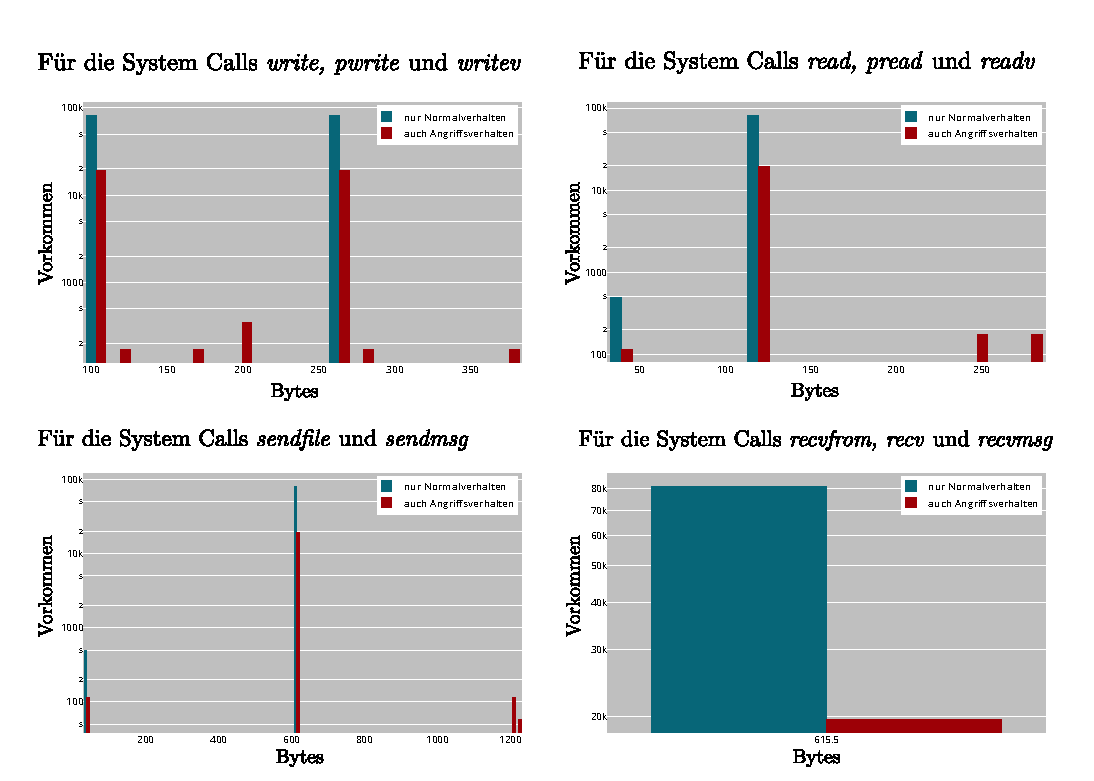
\includegraphics[width=\textwidth]{images/return_2017_plot.pdf}
                        \caption{Histogramm der gelesenen/erhaltenen Bytes für die Testdaten des \ac{LID-DS}~\cite{LID-DS} $CVE-2017-7529$ Szenarios.
                        Dargestellt wird dabei immer der Anteil einer Rückgabewertgröße in Byte an allen Rückgabewertgrößen der besagten System Calls.
                        Links oben für die von den System Calls \textit{write, pwrite} und \textit{writev} geschriebenen Bytes.
                        Rechts oben für die von \textit{read, pread} und \textit{readv} gelesenen Bytes.
                        Links unten für die von \textit{sendfile} und \textit{sendmsg} über Sockets gesendete Bytes.
                        Rechts unten für die von \textit{recvfrom, recv} und \textit{recvmsg} über Sockets erhaltenen Bytes.
                        Blau: Nur Normalverhalten, Rot:Normalverhalten und Angriffsverhalten}
                        \label{fig:return_values}
                    \end{figure}

        \subsection{Darstellung eines System Call Streams}\label{sec:streamdarstellung}
            Nachdem die Kodierung eines System Calls und zwei weiterer Parameter neben dem Namen selbst besprochen wurde, soll in diesem Abschnitt die Abarbeitung mehrerer System Calls für den verarbeitenden Algorithmus behandelt werden.
            Dabei werden die Abfolge der System Calls des Datensatzes als ein kontinuierlicher Stream betrachtet.
            Dies ermöglicht den Einsatz der entwickelten Vorgehensweise in der Praxis auch im Live-Betrieb, sofern die Verarbeitung entsprechend schnell stattfindet.
            Für viele Algorithmen wie zum Beispiel auch neuronale Netze ist es sinnvoll und teilweise unausweichlich eine feste Eingangsgröße festzulegen.
            Um dies für einen Stream zu ermöglichen werden in der \ac{NLP} schon seit langer Zeit n-gramme verwendet~\cite{NGRAMSUEN1979}.
            Auch in der auf System Call basierten Anomalieerkennung kommen n-gramme zum Einsatz~\cite{STIDE_Alternatives, SYSCALL_GRAPHS, IDSTHREADGRIMMER2021}.
            Ein n-gramm ist eine zusammenhängende Folge von $n$ Elementen aus einer gegebenen Eingabe.
            Diese werden wie in der linken Graphik in \autoref{fig:ngram_thread} Beispielhaft dargestellt aufgebaut.

            Dabei wird ein Buffer der Länge $n$ erzeugt, welcher das erste n-gram liefert sofern sich $n$ Elemente in dem Buffer befinden.
            Kommt ein neues Element in den Buffer fällt das älteste heraus.

            Zu beachten ist dabei, dass die Abfolge der System Calls mehrere logische Abfolgen zusammenführt.
            Denn moderne Computer Systeme verarbeiten mehrere Threads parallel.~\cite{SYSCALL_SILBERSCHATZ}
            Die System Calls aller Threads werden dann je nach dem wie sie vom Betriebssystemskernel verarbeitet werden an die Sequenz angefügt.
            
            \paragraph{Thread Awareness}
                Grimmer et al.~\cite{IDSTHREADGRIMMER2021} beschreiben in ihrer Arbeit wie sie die Thread Information der System Calls verwenden um diese verwundenen Sequenzen zu entwirren.
                Dabei wird für jeden Thread ein eigener Buffer erzeugt. 
                Die Ausgabe dieser Buffer wird in der rechten Graphik in \autoref{fig:ngram_thread} veranschaulicht. 
                Also nur System Calls aus demselben Thread bilden ein n-gram.
                Grimmer et al.\ konnten zeigen, dass dies speziell auch für diesen Datensatz eine Verbesserung der Ergebnisse erreicht werden konnte.

                \begin{figure}
                    %thread ngram image
                    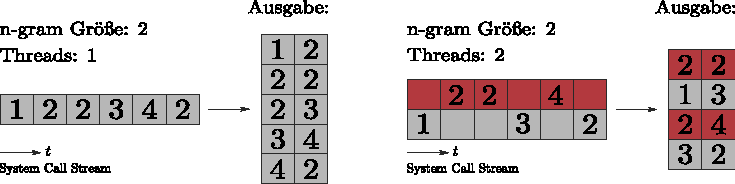
\includegraphics[width=\textwidth]{images/ngram.pdf}
                    \caption{Erstellung der n-gramme mit $n=2$ aus einem Datenstream von System Calls.
                        Links ohne und rechts mit der Beachtung der Threadinformation.
                        Die dabei entstehenden n-gramme dienen als Eingabe für den bewertenden Algorithmus.
                        Die Reihenfolge der entstehenden n-gramme als Eingaben ist dabei von oben nach unten.
                    }\label{fig:ngram_thread}
                \end{figure}

            \paragraph{Thread Change Flag}
                Sie verwenden in der Auswertung aber ausschließlich Algorithmen welche kontextfrei arbeiten.
                Dies bedeutet, dass zuvor gesehene n-gramme keinen Einfluss auf das aktuelle haben.
                Wie in~\autoref{sec:LSTM} beschrieben wird, ist das bei \ac{LSTM} Netzwerken nicht der Fall.
                Es gilt also den benötigten Kontext in die von Grimmer et al.\ beschriebene Methodik zu integrieren.

                Eine Möglichkeit bestünde darin die ThreadID zu kodieren und die Information aus welchem Thread das n-gram stammt mitzugeben.
                Doch das Kodieren der tatsächlichen Thread ID ist sehr unpraktisch, da Thread IDs wiederverwendet werden können.
                Stattdessen wird in dieser Arbeit ein n-gram mit der Informatione über einen Kontextwechsel angereichert. 
                Dieser Kontextwechsel soll dann über die \ac{TCF} an das \ac{LSTM} übergeben werden.
                Initial wird, weil kein Kontextwechsel stattfindet, für die \ac{TCF} eine $0$ angegeben.
                Kommt das aktuelle n-gram aus demselben Thread wie das n-gram zuvor, ist die \ac{TCF} ebenfalls $0$.
                Ist das aktuelle n-gram allerdings aus einem anderen Thread wird ein Kontextwechsel durch das Setzen der \ac{TCF} auf $1$ angezeigt.
                Visualisiert wird dies in \autoref{fig:ngram_tcf}.

                \begin{figure}[ht]
                    %thread ngram image
                    \centering
                    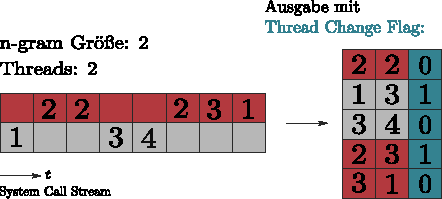
\includegraphics[width=0.6\textwidth]{images/tcf.pdf}
                    \caption{Analog zu \autoref{fig:ngram_thread} werden n-gramme erzeugt.
                             Diese werden nun mit der \ac{TCF} angereichert.
                             Initial ist die \ac{TCF} $0$.
                             Ist das zuvor ausgegeben n-gram aus demselben Thread, ist die \ac{TCF} ebenfalls $0$.
                             Findet ein Wechsel des Threads statt, wird dieser Kontextwechsel durch das Setzen der \ac{TCF} auf $1$ signalisiert.}\label{fig:ngram_tcf}
                \end{figure}

                Die Vorstellung dabei ist, dass eine \ac{TCF}$= 1$ dem \ac{LSTM} die Information gibt, dass der zuvor gesehene n-gramme nur eine untergeordnete Rolle für den Kontext spielen, da diese aus einem anderen Thread stammen.
                Falls dies der Fall ist, kann ein häufiger Kontextwechsel dafür sorgen, dass der Vorteil der \ac{LSTM}s abgeschwächt wird, da immer dafür gesorgt wird, dass potentiell wenige Informationen im Kontext enthalten sind.
                In \autoref{tab:tcf} wird dargestellt wie oft so ein Kontextwechsel stattfindet.
                Dabei ist zu erkennen, dass in den Szenarien aus dem \ac{LID-DS} bei einer Länge von $n=6$ nur bis zu $13.8\%$ der n-gramme eine \ac{TCF}$=1$ haben.
                Die zuvor geschilderte Gefahr scheint also für die gegebenen Szenarien keine Rolle zu spielen, ist aber für andere Einsatzbereiche mit nicht kontextfreien verarbeitenden Algorithmen zu beachten.

                \begin{table}[ht]
                    \small
                    \centering
                    \begin{tabular}{c|c|c|c}
                        \hline
                        \rowcolor{GruvGray!36}
                        \multicolumn{4}{c}{Thread Change Flag}\\
                        \hline
                        Szenario & #\ac{TCF}$=1$ & #\ac{TCF}$=0$ & \makecell{Anteil \ac{TCF}$=1$ \\an allen n-grammen \\ in \%}\\
                        \hline
                        \hline
                        \rowcolor{GruvGray!16}
                        $Bruteforce\_CWE\_307$ & $2534165$ & $20383314$ & $11.1$ \\
                        $CVE-2012-2122$ & $1206151$ & $10365309$ & $10.4$ \\
                        \rowcolor{GruvGray!16}
                        $CVE-2014-0160$ & $1120786$ & $7026864$ & $13.8$ \\
                        $CVE-2017-7529$ & $1130717$ & $10721010$ & $9.5$ \\
                        \rowcolor{GruvGray!16}
                        \hline
                    \end{tabular}
                    \caption{Vorkommen von eines Kontextwechsels angezeigt durch die \ac{TCF}.
                    Bei einer n-gram Länge von $6$}
                    \label{tab:tcf}
                \end{table}

        \section{Aufbau LSTM}\label{sec:aufbau_lstm}
        \begin{figure}[ht]
            \centering
            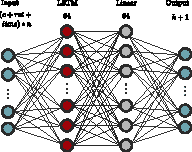
\includegraphics[width=0.7\textwidth]{images/lstm.pdf}
            \caption{Aufbau des \ac{LSTM} mit $64$ Neuronen für die \ac{LSTM}- und Linear-Layer.
                Die Input Layer besitzt $(e + ret + time) * n$ Neuronen, mit $e$ für die Größe des \ac{W2V}-Embeddings,
                $ret=1$ falls Rückgabewerte verwendet werden und $time=1$ falls die Zeitabstände verwendet werden.
                Ansonsten sind $ret=0$ und $time=0$.
                Und die Output Layer hat $k+1$ Ausgangsneuronen, dabei ist $k$ die Anzahl an System Calls aus dem Trainingsdatensatz.
                Eins wird addiert für unbekannte System Calls.}
                \label{fig:lstm}
        \end{figure}

        Der Allgemeine Aufbau des \acp{LSTM} wird in \autoref{fig:lstm} präsentiert.
        Wie dargestellt, wird für die Initialisierung der für diese Arbeit entwickelten Implementierung des \acp{LSTM} die Anzahl an Input und Output Neuronen benötigt.
        Für die Eingangsgröße gilt:
        \begin{equation}
            input\_dim = (e + ret + time) \cdot n
        \end{equation}
        Mit $e$ für die Größe des \ac{W2V}-Embeddings.
        Falls der zuvor beschriebene Zusatzparameter für die Rückgabewerte verwendet wird gilt $ret=1$ ansonsten $ret=0$.
        Gleiches gilt für den Extraparameter welcher die Zeitabstände kodiert.
        Für die Ausgangsgröße gilt:
        \begin{equation}
            output\_dim = k + 1
        \end{equation}
        Dabei ist $k$ die Anzahl an System Calls aus dem Trainingsdatensatz, eins wird addiert für unbekannte System Calls.
        Nötig ist diese Variabilität, da für die Initialisierung des \acp{LSTM} die Anzahl der verschiedenen System Calls im Trainingsdatensatz für die Ausgangsgröße, sowie die Eingangsgröße des System Calls eine Rolle entscheidende Rolle spielt.

        Festgelegt werden hingegen Größen für die \textit{Hidden Layer} Dimension, \textit{Batch Size}, den \textit{Optimizer} die \textit{Loss}-Funktion und die Lernrate.
        Die Dimension der \ac{LSTM}-Layer wird auf $64$ gesetzt, die \textit{Batch Size} auf $1024$.
        Es wird der für \acp{LSTM} gängige \textit{Adam Optimizer} gewählt.
        Da es sich um eine Klassifikation mit $k+1$ Klassen handelt wird die \textit{Cross-Entropy} Loss-Funktion des PyTorch Frameworks genutzt.
        Die Lernrate wird auf $0.001$ festgelegt.

        Die Architektur wird ebenfalls in \autoref{fig:lstm} dargestellt und besteht aus der Eingabe-Layer, der \ac{LSTM}-Layer, einer \textit{fully-connected} Linear-Layer und der Output-Layer.

        Entgegen der typischen Implementierungen von \acp{LSTM} wird der \textit{Hidden State} nach einem Batch gespeichert und dem nächsten Batch  übergeben. 
        Ansonsten würde die Kontextinformation zwischen den Batches verloren gehen.
        Diese Idee ist allerdings ausgelegt für einen kontinuierlichen Stream an System Calls, der Datensatz besteht aber aus vielen Dateien.
        Deswegen wird der \textit{Hidden State} zum Ende einer Aufnahme zurückgesetzt.
        Details zu der Parameterwahl wird in \autoref{sec:parameterwahl} erläutert.

        Ausgaben des \acp{LSTM} sind durch die Verwendung der PyTorch CrossEntropy Loss-Funktion sogenannte \textit{Logits}.
        Auf diese kann mithilfe der \textit{Softmax}-Funktion eine Liste an Wahrscheinlichkeiten für jeden System Call sowie den Platzhalter erstellt werden.

    \section{Algorithmus}\label{sec:Algorithmus}
        Im vorigen Kapitel wurden alle verwendeten Vorverarbeitungsschritte vorgestellt.
        In den kommenden Abschnitten werden diese Schritte zu einem Ablauf zusammengeführt.
        Zunächst soll in \autoref{sec:Allgemein} ein allgemeiner Überblick gegeben werden.
        Anschließend wird in \autoref{sec:Training} behandelt was das \ac{LSTM} Netzwerk lernt.
        Wie aus dem Gelernten dann die Einstufung in Normal- oder Angriffsverhalten stattfindet, wird dann in \autoref{sec:Anomalieerkennung} und \autoref{sec:Schwellung}.
        Abschließend werden dann grobe Richtlinien für die Parameterwahl in \autoref{sec:StrukExp} erstellt.

        \subsection{Allgemein}\label{sec:Allgemein}
            Wie bereits in \autoref{sec:related_nlp} beschrieben, werden verschiedene Verfahren der \ac{NLP} auch in der anomaliebasierten \ac{HIDS} eingesetzt.
            Neben den bereits beschriebenen \ac{W2V} Verfahren kommen auch die in der \ac{NLP} verbreiteten \ac{LSTM} Netzwerke zum Einsatz.
            Mit dem \ac{LSTM} soll in der Trainingsphase ein Sprachmodell der System Calls erstellt werden.
            Anhand dieses Modells soll dann in der Testphase eine Vorhersage über den nächsten System Call gemacht werden.
            Diese Vorhersage besteht aus den Wahrscheinlichkeiten für alle aus dem Training gesehenen System Calls, plus einem Platzhalter für noch unbekannte System Calls.
            Die Wahrscheinlichkeit des tatsächlich auftretenden System Calls stellt dann den Anomaliescore dar.
            Ob dieser Anomaliescore zu einem Alarm führt oder nicht, hängt von einem zuvor bestimmten Schwellwert ab.
            Dieser wird bestimmt, indem nach dem Training die Anomaliescores für einen Ausschnitt des Datensatzes bestimmt werden.
            In diesem Ausschnitt, auch Validierungsdaten genannt, darf kein Angriffsverhalten enthalten sein.
            Eine Garantie die in der echten Welt nie komplett gegeben werden kann.
            In den Validierungsdaten soll folglich kein Alarm ausgelöst werden, weshalb der höchste Anomaliescore der Validierungsdaten als Schwellwert der Anomalieerkennung verwendet wird.
            Dies ist definitiv nur eine Annäherung an einen optimalen Schwellwert.

            Die System Calls werden wie zuvor beschrieben durch das \ac{W2V} Verfahren in einen Vektor umgewandelt und durch die zwei zuvor beschriebenen Verfahren, die Normalisierung der Zeitabstände und der Rückgabewerte bestimmter System Calls, angereichert.
            Der Stream der System Calls wird dann mit Betrachtung der Threads in n-gramme zusammengetragen.
            Zusätzlich wird zu jedem n-gram die Information über einen Kontextwechsel durch die \ac{TCF} angegeben.
            % Im Folgenden wird der Trainingsablauf detaillierter bestimmt.

        \subsection{Training}\label{sec:Training}
            \begin{figure}
                \centering
                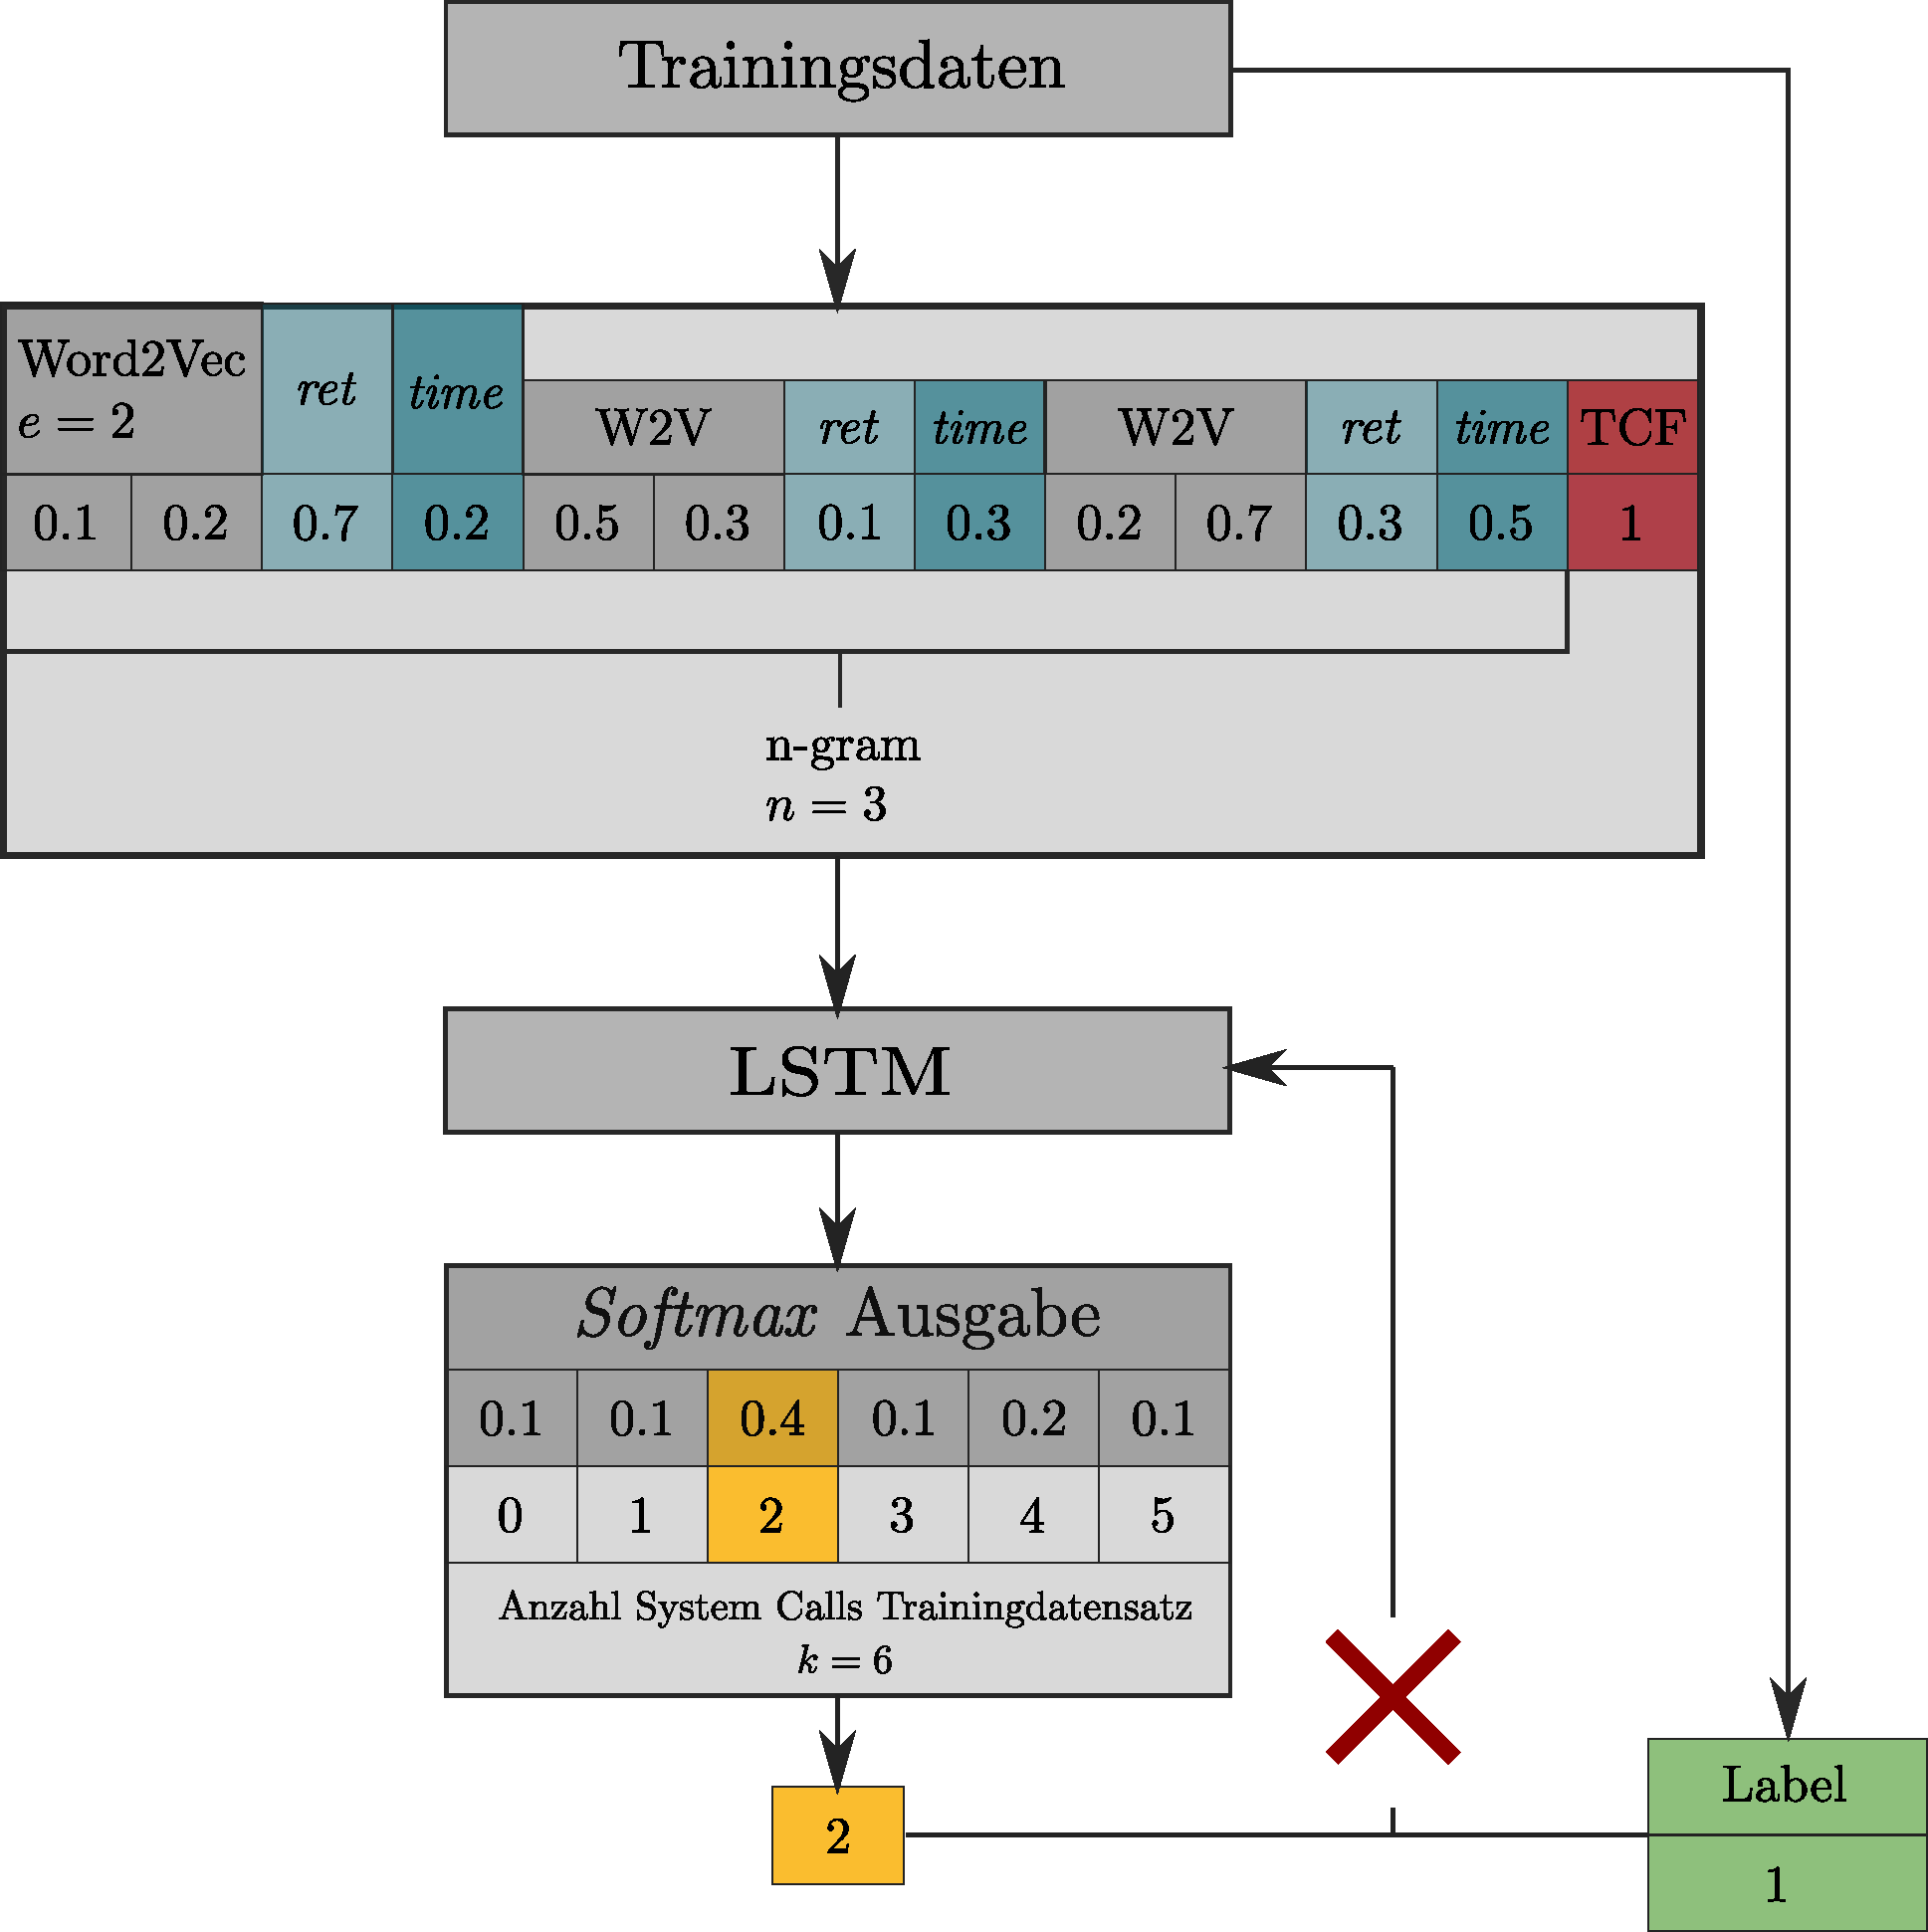
\includegraphics[width=0.75\textwidth]{images/Process_overview.pdf}
                \caption{Ablauf der Trainingsphase mit Beispieldaten.
                        Aus Trainingsdaten wird ein n-gram aus \ac{W2V}, Rückgabewert (\textit{ret}) und Zeitabstand (\textit{time}) erstellt.
                        Diese beiden Extraparameter sind bläulich hervorgehoben.
                        Zusätzlich wird die \ac{TCF} an das n-gram gefügt.
                        Der Index des höchsten Wertes (gelb) aus der Ausgabe des \ac{LSTM} wird mit dem eigentlichen Label (grün) verglichen.
                        Aufgrund dieser Information werden die Gewichte im \ac{LSTM} angepasst}
                        \label{fig:training}
            \end{figure}
            % Für das Training des \ac{LSTM} Netzwerkes werden nur Normaldaten aus dem Trainingsdatensatz verwendet.
            Pro Szenario werden $200$ der ca.\ $1100$ Aufnahmen welche nur Normalverhalten enthalten für das Training ausgewählt.
            Die Grundidee besteht darin mit einer gegebenen Sequenz $s = (sc_{x_1},\dots,sc_{x_n})$, in diesem Fall ein n-gram, den folgenden System Call $sc_{x_{n+1}}$ vorherzusagen. 
            Da der nächste System Call aus dem Datensatz stets bekannt ist, kann als Feedback für das Netzwerk die Information genommen werden ob $sc_{x_{n+1}}$ korrekt vorhergesagt wurde.
            Diese lässt sich durch die folgende Formel beschreiben.
            \begin{equation}
                P\left(x_i|x_{1:i-1}\right) \forall i
            \end{equation}
            Das \ac{LSTM} gibt wie in \autoref{fig:training} dargestellt diese Information an das \ac{LSTM} zurück.

            Seien die System Calls aus den Trainingsdaten aus der Menge $SC = \{sc_1,sc_2,\dots,sc_k\}$.
            Womit $k$ die Anzahl der in den Trainingsdaten vorkommenden System Call Namen angibt.
            Durchlaufe Trainingsdaten und erstelle n-gramme $ngram_i$ und verwende den auf das n-gram folgenden System Call als Label $l_i$.
            Danach ist das erste n-gram $ngram_0$ mit Label $l_0$.
            Dabei werden die System Call Namen durch Integerwerte ersetzt. 
            Das \ac{LSTM} Netzwerk bekommt $ngram_0$ und gibt einen Vektor der Länge $k+1$ zurück.
            Damit für jeden der $k$ möglichen System Calls aus den Trainingsdaten eine Auftrittswahrscheinlichkeit angegeben.
            Zusätzlich wir $1$ addiert, da in den Testdaten unbekannte System Calls auftreten können.
            Diese bekommen den \ac{W2V}-Vektor $(0,0)$ und einen Integerwert von $0$. 
            Die Ausgabe des \acp{LSTM} sind \textit{Python Logits}, diese werden mithilfe der \textit{Softmax}-Funktion in die gewünschten Wahrscheinlichkeiten umgewandelt.
            Der Index der Liste der Wahrscheinlichkeiten wird mit dem aus den Trainingsdaten gezogenen Label verglichen.
            Dieser Vergleich dient dann als Feedback für das \ac{LSTM}.
            Mit den gegebenen Trainingsdaten kann nun das \ac{LSTM} mittels des \textit{back-propagation through time}  trainiert werden.

            Wird mit \ac{W2V} zu $V_{sc} = \{v_{sc1},v_{sc2},\dots,v_{scn}\}$.
            
            Gab es in den Trainingsdaten die feste Menge $S = \{1,\dots,N\}$ an System Calls, so gibt $x=x_1\dots x_l \ (x_i\in S)$ die Sequenz an $l$ System Calls an.
            Jeder dieser System Calls bekommt im ersten Schritt einen Integerwert zwischen 1 und $N$.
            Taucht in den Testdaten nun ein noch nicht bekannter System Call $x_i$ auf, also $x_i \notin S$, so erhält dieser den vorläufigen Wert 0.
            Zu jedem Zeitpunkt wird $x_i$ der Input Layer übergeben.
            Dabei wird ein Embedding aus Abschnitt~\ref{sec:embedding} verwendet. 
            An der Ausgangs Layer befindet sich eine Softmax Aktivierungsfunktion.
            Diese wird verwendet um die Ausgabe zu normalisieren und damit die Wahrscheinlichkeitsverteilung des nächsten System Calls zu erhalten.
            % Im ersten Schritt besteht dieses Embedding aus dem \textit{One hot encoding} (OHE).
            % In weiterer Ausführung werden dann zwei W2V Verfahren verwendet.
            % Wie in Kapitel \ref{Grundlagen:LSTM} bereits beschrieben wird, soll das LSTM mit den kodierten system calls aus dem Trainingsdatensatz trainiert werden.

        \subsection{Anomalieerkennung}\label{sec:Anomalieerkennung}
            \begin{figure}
                \centering
                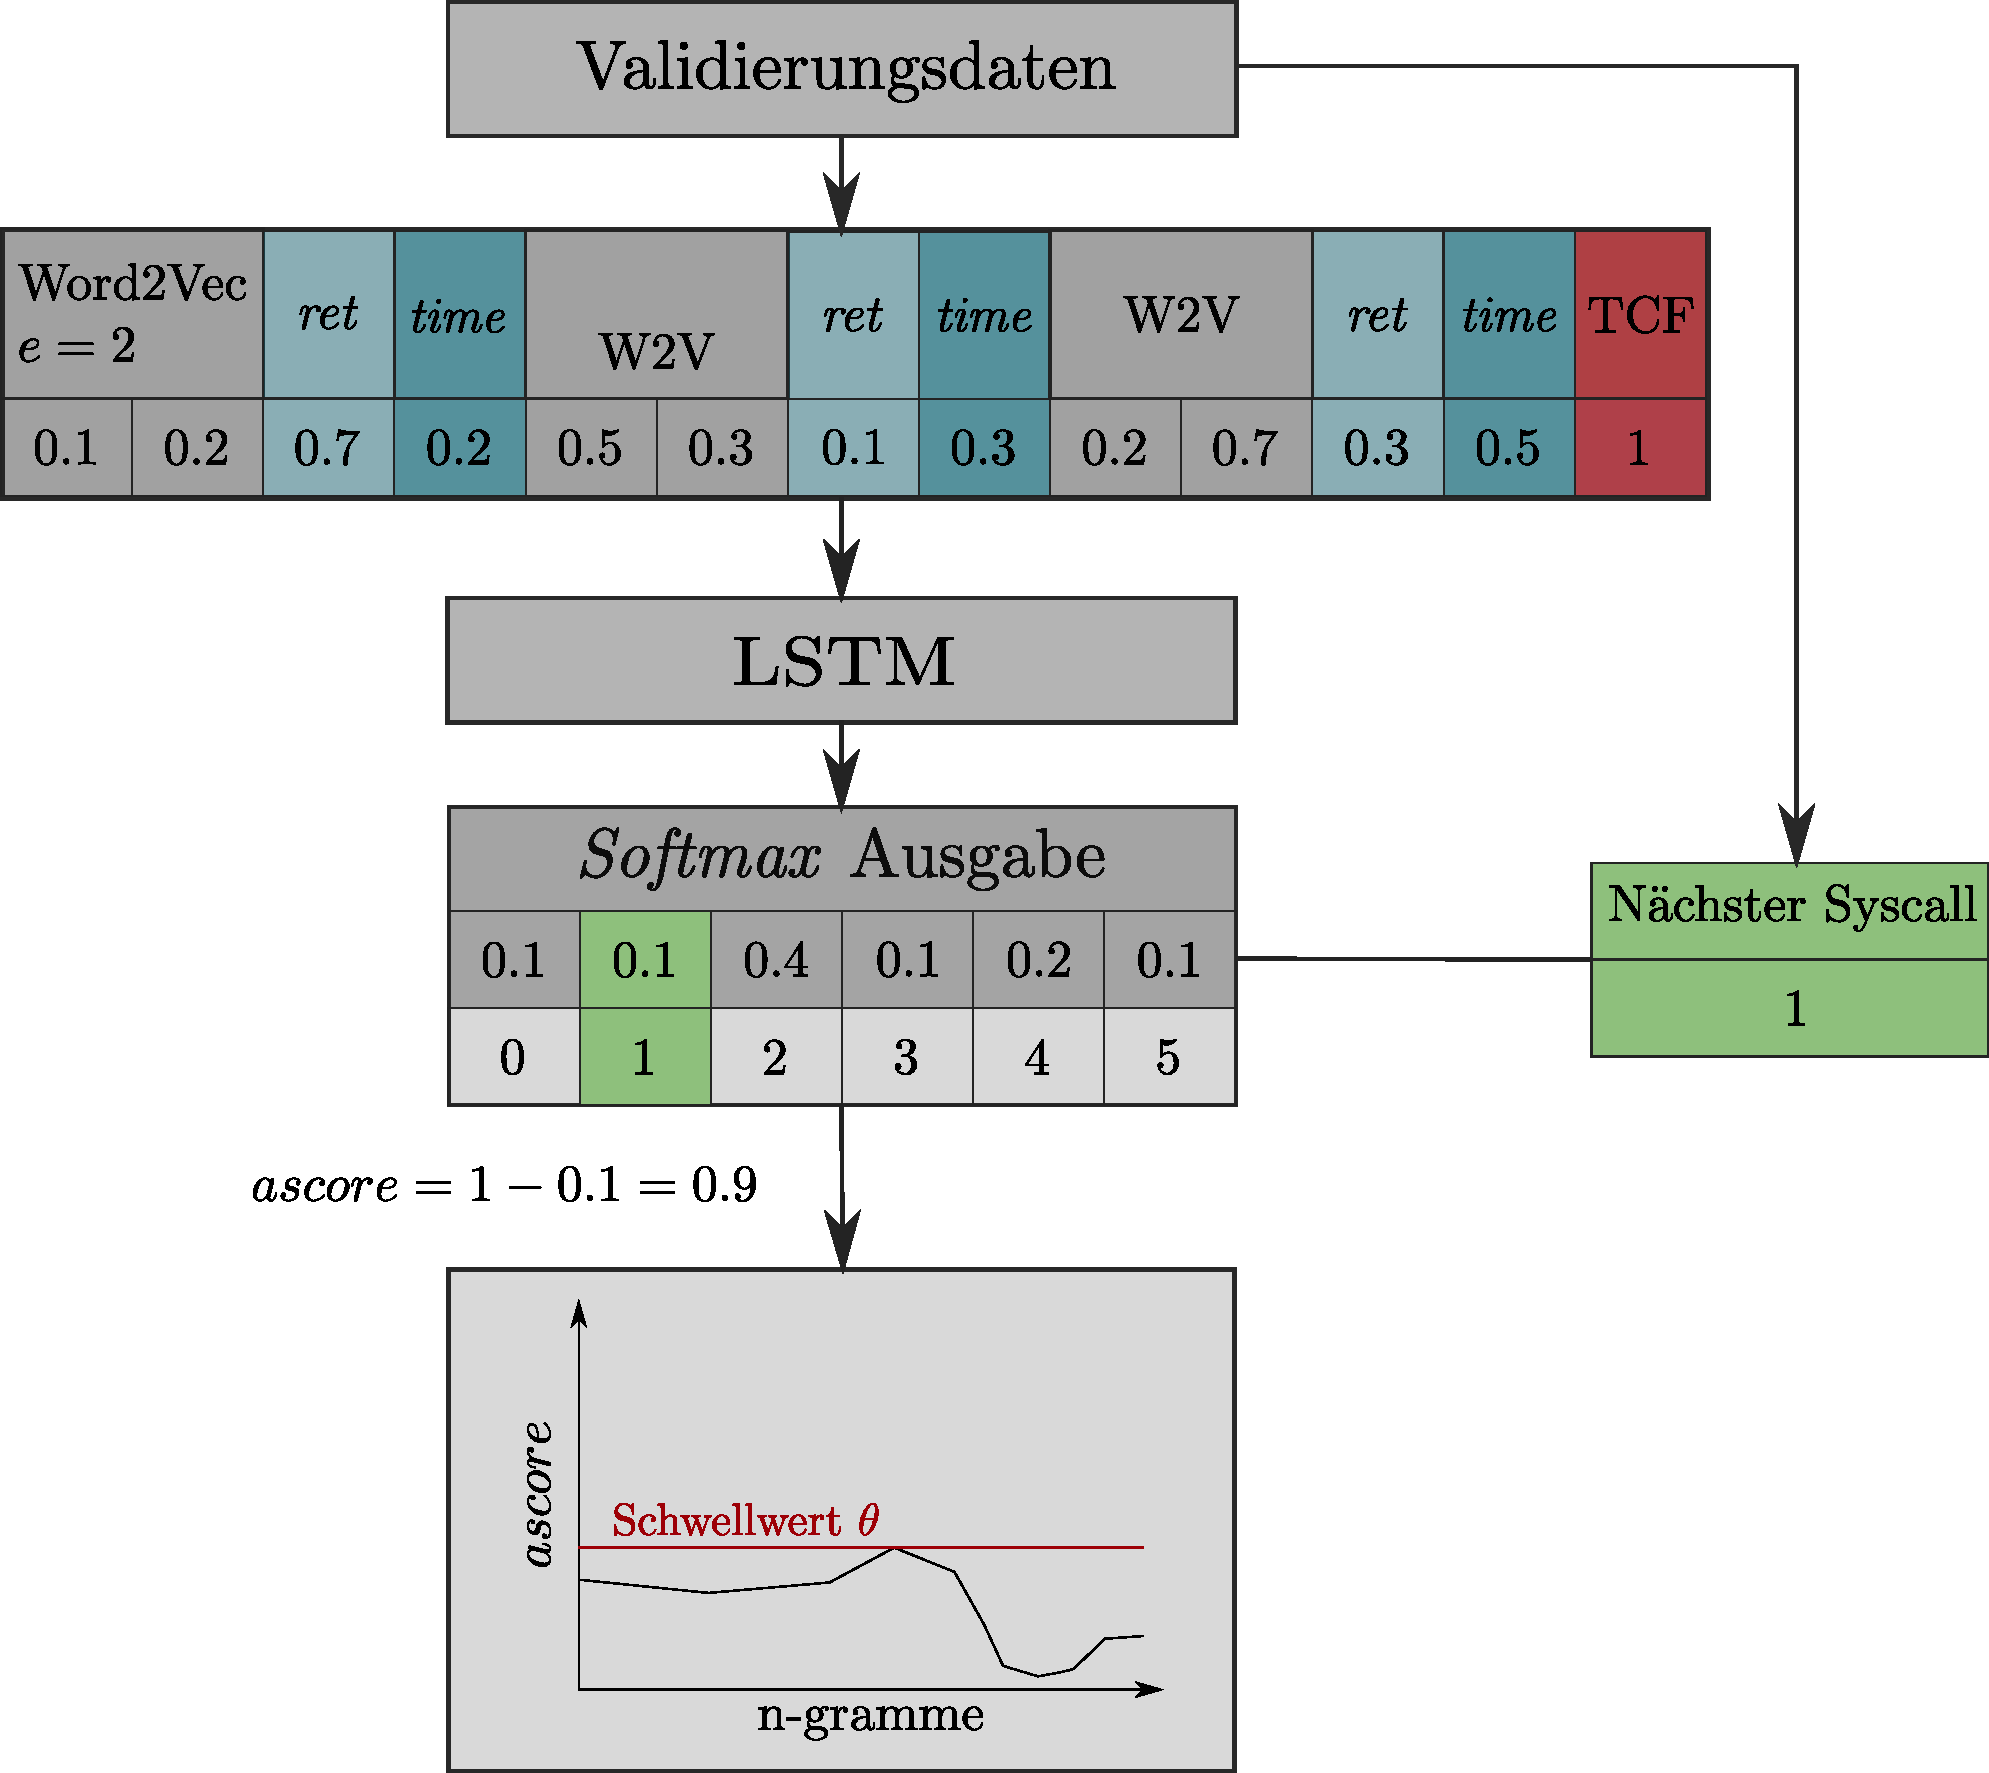
\includegraphics[width=0.7\textwidth]{images/Validation_overview.pdf}
                \caption{}
                \label{fig:training}
            \end{figure}
            Es kann also bei Auftreten des System Calls $x_i$ überprüft werden mit welcher Wahrscheinlichkeit $p$ dieser vorhergesagt wurde.
            Der eigentliche Anomalie-Score wird dann folgenderweise berechnet:
            \begin{equation}
                ascore = 1 - p
            \end{equation}
            Unterschreitet dieser einen Schwellwert so wird dies als eine Anomalie gewertet und ein Alarm angezeigt.
            \subsection{Schwellwertbestimmung}\label{sec:Schwellung}
            Um den zuvor erwähnten Schwellwert automatisch zu bestimmen, wird der Algorithmus auf die Validierungsdaten angewendet. 
            Dabei dient der höchste Wert dieser Daten dann als Schwellwert, da angenommen wird, dass mindestens alle Daten aus den Validierungsdaten harmlos sind und damit unter dem Schwellwert liegen sollten.
            Wichtig ist dabei dafür nicht die Trainingsdaten zu wählen, da eine starke Verzerrung der Schwellwertes durch Overfitting der Daten entstehen kann. 
            Das würde bedeuten, dass nur sehr geringe Anomaliewerte auftreten und der Schwellwert sehr gering ist und damit die Gefahr für viele Fehlalarme besteht.

            Alternativ betrachte die x wahrscheinlichsten vorhergesagten system calls, falls tatsächlicher system call nicht dabei --> alarm.
            X ermitteln, betrachte validierungsdaten und schaue ob schlechtestes x aussehen würde.
            Tatsächlich oft einmal schlechteste platzierung und automatische erkennung von x schwer.

        \subsection{Parameterwahl}\label{sec:parameterwahl}
            ngram länge.
            lstm merkt sich vorherige syscalls aber hinzunahme von syscalls weitere info.
            -> finden von sweet spot.
            wichtiger Parameter den es zu ermitteln gilt.

    \section{Strukturierung der Experimente}\label{sec:StrukExp}
        Um aussagekräftige Experimente zu entwickeln müssen zuerst 
        überlegungen zur praktischen umsetzung gemacht werden
        dabei wird in ersten Tests klar, dass zeit hierbei eine große rolle spielen wird

        erste Tests also ausgelegt um Faktoren zu ermitteln, welche die auswertungen stark verlangsamen
        und diese ausschließen.

        \subsection{Faktor Zeit}

            zeit/dr als groesse und farbe von scatter plot
            batch size test und train x/y achse

            eingrenzen von moeglichen konfigurationen

            Berechnungszeiten aus verschiedenen Perspektiven relevant:
            soll live system werden
            begrenzte rechenleistung und viele Tests zur auswertung von parametern architektur etc
            erster test zur abschätzung diverser zeitl.\ faktoren:

            Faktoren:
            \begin{itemize}
                \item Architektur
                \item Verarbeitung Stream

                     ngram größe
                \item embedding
            \end{itemize}
        ngram größe, architektur und verwendung w2v statt ohe
        Grobe Abschätzung der Zeit, da Berechnungen auf Clustern ausgeführt werden von Auslastung beeinflusst werden.
        Klare Erkenntnisse:

            Single Small 50 neuronen eine schicht:
            Single Big 250 neuronen eine schicht
            multi 50 neuronrn 3 schichten

        erste Abschätzung von Nutzen von Thread 
        einführen von stateful sowie Batch Normalization

    \subsection{Optimale Parameter}
        \paragraph{Architektur}
            versch architekturen:
            Single Small 50 neuronen eine schicht
            Single Big 250 neuronen eine schicht
            multi small 20 neuronen 3 schichten
            multi big 50 neuronrn 3 schichten
            deep erste 50 sonst 20 6 schichten

            singlesmall 43\% von Deep
            insgesamt am schnellsten single small
            wie zu erwarten,  deep am langsamsten

            teste eine schicht viele neuronen 
            eine schicht wenige neuronen
            mehrere schichten mehrere neuronen / mit dropout dazwischen
            viele schichten wenige neuronen /mit dropout dazwischen

            auf Grund des zeitlichen Faktors fallen Deep und multibig weg
            Also zu testen:
            Single Small
            Single 
            Multi Small
            Multi 

        \paragraph{Hyperparameter}
            aktivierungs funktion
            -> dense layer with softmax or tanh
            batch size
            learning rate
            optimizer

        \paragraph{Ngram Größe}
            ngram größer -> langsamer

        \paragraph{Threadinfo}
            Hypothese:
            Threadinfos bringen was

            Einbinden von thread information auf verschiedenen wegen:
            Thread aware ngrams (tan)
            Thread aware ngrams for w2v (tanw2v)
            Thread change flag (tcf)

            varianten:
            tan
            tanw2v
            tcf
            tan tcf
            tan tanw2v
            tcf tanw2v
            tan tanw2v tcf

            ---> welcher dieser varianten am besten?

        \paragraph{Parameter}
            args
            time

            \ac{LSTM} ohne Threadinfos mit OHE
            LSTM mit W2V ohne Threadinfos (ngram)
            LSTM mit W2V mit Threadinfos (ngram)
            LSTM mit W2V threadaware mit Threadinfos (ngram)
            LSTM mit W2V threadaware mit Threadinfos (ngram) und threadchangeflag
            LSTM mit W2Vthreadaware mit Threadinfos (ngram) und threadchangeflag, spezialtraining
            --> LSTM final

            Manche angriffe verändern Sequenz von syscalls nicht
            Hypothese:
            verwende Parameter um erg zu verb

            LSTM final + strlen
            LSTM final + time delta
            LSTM final + strlen + time delta



\section{Metriken}\label{sec:Metriken}

    Auf Grund dessen Metrik False Alarm/ consecutive false alarm und Detection rate falls einmal pro malicious file in quadrant 4 -> HIT
    Wahl von Metriken in NN
    Precision, Recall, f-score, TNR, FNR, FPR

    problematisch:
    nicht auf systemcall genau gelabelt
    recall precision usw nur auf file ebene:
    alarm nach exploitstarttime wird immer als hit gewertet -> aber evtl angriff noch nicht begonnen
    oder angriff bereits vorbei
    ebenso umgekehrt, eig muss jeder nicht alarm nach exploitstart als FN gewertet werden
    weswegen filegenau geschaut wird
    vorteil des Datensatzes gegenüber anderen, immerhin exploitstart time

    ilarm in quadrant ---> image
